% Copyright 2025 Kieran W Harvie. All rights reserved.

\chapter{The Model}
This project is the exploration of my third toy model of a neural network.
The first two models were lacking in features and notation,
but third times the charm and I'm pretty happy with this attempt:

%\begin{quote}
%A neuron is the ordered pair of a real number and a differentiable real-valued function where the function can have any number of real variables.  
%
%A neural network is a finite partially ordered set of neurons such that:
%There is a bijection between every neuron strictly less than a given neuron and a variable of the given neuron's function.
%And the neuron's real number is equal to to the neuron's function when the corresponding lesser neuron's values are substituted in.
%\end{quote}
\begin{quote}
A neural network $N$ over a commutative ring with unity $K$ is a partial ordering of functions $n:K^{M_n}\rightarrow K$ such that $M_n$ is the set of all functions strictly less than $n$.

A neural network $N$ over $\mathbb{R}$ where all functions $n\in N$ are differentiable is a differentiable neural network.
\end{quote}
This model was arrived at by working backwards to find the most motivated definitions that enable a rich incident algebra,
of the neural network over $\mathbb{R}$,
and ensures that there's an element of the algebra which encapsulated the connection between the neurons.
More on the incident algebra in the next section because I first want to go over the features and limitations of this model.

\subsubsection{Terminology:}
neuron and connection

\subsubsection{Functions and Graphs:}
\[\tilde{n}:K^M\rightarrow K\]
\[
	\tilde{n}(x) = \begin{cases} x_n & n\in M\\ n((\tilde{m}(x))_{m\in M_n}) & n\notin M\end{cases}
\]
Could restrict to $\tilde{M}_n = M\cap M_n$
Well definedness by induction on the size of $M_n$.
There's two points of redundancy in the model.
around a neuron having both a real number and a function.

\subsubsection{Covering, Grading, and Hasse:}
\begin{center}
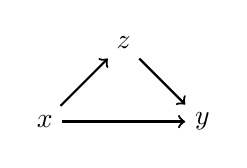
\begin{tikzpicture}
	\node (y) at (2,0) {$y$};
	\node (x) at (0,0) {$x$};
	\node (z) at (1,1) {$z$};
	\draw[->,thick] (x)--(z);
	\draw[->,thick] (x)--(y);
	\draw[->,thick] (z)--(y);
\end{tikzpicture}
\quad
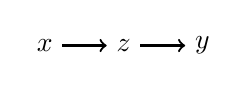
\begin{tikzpicture}
	\node (y) at (2,0) {$y$};
	\node (x) at (0,0) {$x$};
	\node (z) at (1,0) {$z$};
	\draw[->,thick] (x)--(z);
	\draw[->,thick] (z)--(y);
\end{tikzpicture}
\end{center}

They can be represented like a Hasse diagram
covering 
There's soome 

\subsubsection{Differentiability Isn't Sufficient:}

\subsubsection{Maximal and Minimal Elements:}
Error

\subsubsection{The Previous Models:}
Finite double sequence of functions indexed by $I\times J$.
Implicit covering and grading leading to Easy proofs:
\[\frac{\partial \phi_{i+n,j}}{\partial \phi_{i,j}} = \sum_{l\in J}\frac{\partial \phi_{i+n,j}}{\partial \phi_{i+1,l}}\frac{\partial \phi_{i+1,l}}{\partial \phi_{i,j}}\]
Regular chain rule,inductive,swap order,regular chainrule
\[\begin{aligned}
	\frac{\partial \phi_{i+n,j}}{\partial \phi_{i,j}} &= \sum_{m\in J}\frac{\partial \phi_{i+n,j}}{\partial \phi_{i+n-1,m}}\frac{\partial \phi_{i+n-1,m}}{\partial \phi_{i,j}}\\
	&= \sum_{m\in J}\frac{\partial \phi_{i+n,j}}{\partial \phi_{i+n-1,m}}\left(\sum_{l\in J}\frac{\partial \phi_{i+n-1,k}}{\partial \phi_{i+1,l}}\frac{\partial \phi_{i+1,l}}{\partial \phi_{i,j}}\right)\\
	&= \sum_{l\in J}\frac{\partial \phi_{i+1,l}}{\partial \phi_{i,j}}\left(\sum_{m\in J}\frac{\partial \phi_{i+n-1,k}}{\partial \phi_{i+1,l}}\frac{\partial \phi_{i+n,j}}{\partial \phi_{i+n-1,m}}\right)\\
	&= \sum_{l\in J}\frac{\partial \phi_{i+1,l}}{\partial \phi_{i,j}}\frac{\partial \phi_{i+n,j}}{\partial \phi_{i+1,l}}\\
\end{aligned}\]
